
\documentclass[10pt,a4paper]{article}
\usepackage[T1]{fontenc}
\usepackage{tikz}
\usepackage[margin=1cm]{geometry}
\begin{document}

\title{Binary Serach Tree Traversal Algorithms}
\author{}
\date{}
\maketitle

\section*{Introduction}
This document provides a visual representation of binary search tree traversal algorithms. We will explore three different traversal methods: pre-order, in-order, and post-order. Each method is demonstrated through a series of figures that show the binary tree at various stages of traversal.

\section*{Traversal Algorithms}
\begin{itemize}
    \item \textbf{Pre-order Traversal:}
    In pre-order traversal, the nodes are recursively visited in the following order: root, left subtree, right subtree. This traversal method is useful for creating a prefix expression of the tree.
    
    \item \textbf{In-order Traversal:}
    In in-order traversal, the nodes are recursively visited in this order: left subtree, root, right subtree. This method is particularly useful for binary search trees (BSTs) as it retrieves the nodes in ascending order.
    
    \item \textbf{Post-order Traversal:}
    In post-order traversal, the nodes are recursively visited in the order: left subtree, right subtree, root. This traversal method is useful for deleting nodes or evaluating postfix expressions.
\end{itemize}

\section*{Initial Tree State}
The following figure shows the initial state of the binary search tree before any traversal has occurred. This provides a baseline for understanding how the tree changes during traversal.


\begin{figure}[h!]
\centering
\begin{minipage}{0.8\textwidth}
    \centering
    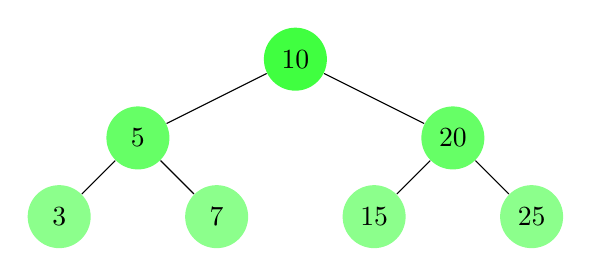
\begin{tikzpicture}[level distance=10mm]
        \tikzstyle{every node}=[fill=green!75,circle,inner sep=1pt, minimum size=8mm]
        \tikzstyle{level 1}=[sibling distance=40mm, set style={{every node}+=[fill=green!60]}]
        \tikzstyle{level 2}=[sibling distance=20mm, set style={{every node}+=[fill=green!45]}]
        \tikzstyle{level 3}=[sibling distance=15mm, set style={{every node}+=[fill=green!30]}]
        \tikzstyle{level 4}=[sibling distance=10mm, set style={{every node}+=[fill=green!15]}]
        \node {10} child {node {5} child {node {3} } child {node {7} }} child {node {20} child {node {15} } child {node {25} }};
    \end{tikzpicture}
    \caption{Initial Tree State}
\end{minipage}
\vspace{1cm}
\end{figure}

\begin{figure}[h!]
\centering

\begin{minipage}{0.8\textwidth}
    \centering
    
\begin{tikzpicture}[level distance=10mm]
        \tikzstyle{every node}=[fill=green!75,circle,inner sep=1pt, minimum size=8mm]
        \tikzstyle{level 1}=[sibling distance=40mm, set style={{every node}+=[fill=green!60]}]
        \tikzstyle{level 2}=[sibling distance=20mm, set style={{every node}+=[fill=green!45]}]
        \tikzstyle{level 3}=[sibling distance=15mm, set style={{every node}+=[fill=green!30]}]
        \tikzstyle{level 4}=[sibling distance=10mm, set style={{every node}+=[fill=green!15]}]
        \node[fill=olive!60] {3} ;
    \end{tikzpicture}
    \caption{Step 2}
\end{minipage}
\vspace{1cm}

\begin{minipage}{0.8\textwidth}
    \centering
    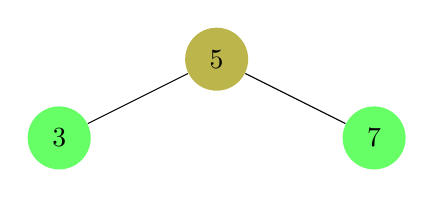
\begin{tikzpicture}[level distance=10mm]
        \tikzstyle{every node}=[fill=green!75,circle,inner sep=1pt, minimum size=8mm]
        \tikzstyle{level 1}=[sibling distance=40mm, set style={{every node}+=[fill=green!60]}]
        \tikzstyle{level 2}=[sibling distance=20mm, set style={{every node}+=[fill=green!45]}]
        \tikzstyle{level 3}=[sibling distance=15mm, set style={{every node}+=[fill=green!30]}]
        \tikzstyle{level 4}=[sibling distance=10mm, set style={{every node}+=[fill=green!15]}]
        \node[fill=olive!60] {5} child {node {3} } child {node {7} };
    \end{tikzpicture}
    \caption{Step 3}
\end{minipage}
\vspace{1cm}

\begin{minipage}{0.8\textwidth}
    \centering
    
\begin{tikzpicture}[level distance=10mm]
        \tikzstyle{every node}=[fill=green!75,circle,inner sep=1pt, minimum size=8mm]
        \tikzstyle{level 1}=[sibling distance=40mm, set style={{every node}+=[fill=green!60]}]
        \tikzstyle{level 2}=[sibling distance=20mm, set style={{every node}+=[fill=green!45]}]
        \tikzstyle{level 3}=[sibling distance=15mm, set style={{every node}+=[fill=green!30]}]
        \tikzstyle{level 4}=[sibling distance=10mm, set style={{every node}+=[fill=green!15]}]
        \node[fill=olive!60] {7} ;
    \end{tikzpicture}
    \caption{Step 4}
\end{minipage}
\vspace{1cm}

\begin{minipage}{0.8\textwidth}
    \centering
    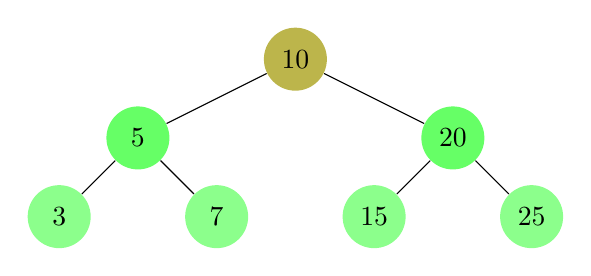
\begin{tikzpicture}[level distance=10mm]
        \tikzstyle{every node}=[fill=green!75,circle,inner sep=1pt, minimum size=8mm]
        \tikzstyle{level 1}=[sibling distance=40mm, set style={{every node}+=[fill=green!60]}]
        \tikzstyle{level 2}=[sibling distance=20mm, set style={{every node}+=[fill=green!45]}]
        \tikzstyle{level 3}=[sibling distance=15mm, set style={{every node}+=[fill=green!30]}]
        \tikzstyle{level 4}=[sibling distance=10mm, set style={{every node}+=[fill=green!15]}]
        \node[fill=olive!60] {10} child {node {5} child {node {3} } child {node {7} }} child {node {20} child {node {15} } child {node {25} }};
    \end{tikzpicture}
    \caption{Step 5}
\end{minipage}
\vspace{1cm}

\begin{minipage}{0.8\textwidth}
    \centering
    
\begin{tikzpicture}[level distance=10mm]
        \tikzstyle{every node}=[fill=green!75,circle,inner sep=1pt, minimum size=8mm]
        \tikzstyle{level 1}=[sibling distance=40mm, set style={{every node}+=[fill=green!60]}]
        \tikzstyle{level 2}=[sibling distance=20mm, set style={{every node}+=[fill=green!45]}]
        \tikzstyle{level 3}=[sibling distance=15mm, set style={{every node}+=[fill=green!30]}]
        \tikzstyle{level 4}=[sibling distance=10mm, set style={{every node}+=[fill=green!15]}]
        \node[fill=olive!60] {15} ;
    \end{tikzpicture}
    \caption{Step 6}
\end{minipage}
\vspace{1cm}

\begin{minipage}{0.8\textwidth}
    \centering
    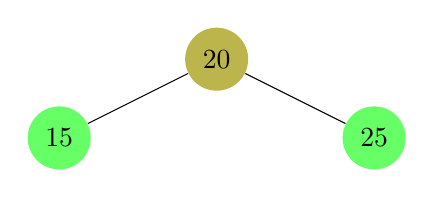
\begin{tikzpicture}[level distance=10mm]
        \tikzstyle{every node}=[fill=green!75,circle,inner sep=1pt, minimum size=8mm]
        \tikzstyle{level 1}=[sibling distance=40mm, set style={{every node}+=[fill=green!60]}]
        \tikzstyle{level 2}=[sibling distance=20mm, set style={{every node}+=[fill=green!45]}]
        \tikzstyle{level 3}=[sibling distance=15mm, set style={{every node}+=[fill=green!30]}]
        \tikzstyle{level 4}=[sibling distance=10mm, set style={{every node}+=[fill=green!15]}]
        \node[fill=olive!60] {20} child {node {15} } child {node {25} };
    \end{tikzpicture}
    \caption{Step 7}
\end{minipage}
\vspace{1cm}

\end{figure}
\newpage

\begin{figure}[h!]
\centering

\begin{minipage}{0.8\textwidth}
    \centering
    
\begin{tikzpicture}[level distance=10mm]
        \tikzstyle{every node}=[fill=green!75,circle,inner sep=1pt, minimum size=8mm]
        \tikzstyle{level 1}=[sibling distance=40mm, set style={{every node}+=[fill=green!60]}]
        \tikzstyle{level 2}=[sibling distance=20mm, set style={{every node}+=[fill=green!45]}]
        \tikzstyle{level 3}=[sibling distance=15mm, set style={{every node}+=[fill=green!30]}]
        \tikzstyle{level 4}=[sibling distance=10mm, set style={{every node}+=[fill=green!15]}]
        \node[fill=olive!60] {25} ;
    \end{tikzpicture}
    \caption{Step 8}
\end{minipage}
\vspace{1cm}

\end{figure}
\newpage

\end{document}
